\documentclass{article}
\usepackage{iclr2026_conference,times}
\input{math_commands.tex}

\usepackage{graphicx}
\usepackage{booktabs}
\usepackage{hyperref}
\usepackage{url}

\iclrfinalcopy

\title{Reproducing and Extending PiSSA-LoRA for Vision Transformer Fine-Tuning on CIFAR-10}

\author{
Muttaqi Ahmad Alladin \\
Department of Statistics and Computer Science \\
Purdue University \\
West Lafayette, IN, USA
}

\begin{document}

\maketitle

\begin{abstract}
Parameter-efficient fine-tuning is attractive for vision models because full fine-tuning updates tens of millions of parameters even for relatively small downstream tasks. This project studies whether PiSSA initialization, originally proposed for low-rank adaptation in language models, also improves adapter-based fine-tuning for image classification. We compare linear probing, full fine-tuning, standard LoRA, and PiSSA-LoRA on a pre-trained Vision Transformer using CIFAR-10. Beyond a direct reproduction-style comparison, we extend the study with multi-seed evaluation, data-regime sweeps, and rank ablations. PiSSA-LoRA achieves the best mean validation accuracy in every suite. In the quick ablation on 5k training images, PiSSA-LoRA reaches 97.53\% mean best validation accuracy while training only 0.351\% of the model parameters, outperforming both standard LoRA and full fine-tuning. In the data-regime study, PiSSA-LoRA consistently beats LoRA from 1k through 50k training examples, with its largest gain appearing in the 1k low-data regime. Code and \LaTeX{} sources are available at \href{https://github.com/muttaqiahmadalladin/ECE5700/tree/main}{the project repository}.
\end{abstract}

\section{Introduction}

Large pre-trained vision backbones transfer well, but adapting them by full fine-tuning is still expensive because every downstream task updates the entire model. Vision Transformers (ViTs) are especially appealing for transfer learning because the same backbone can support many image tasks with minimal architectural changes \citep{dosovitskiy2021vit}. However, full fine-tuning a ViT updates more than 85 million parameters in our setup, which is unnecessary for small datasets such as CIFAR-10.

Low-Rank Adaptation (LoRA) addresses this problem by freezing the backbone and learning small low-rank updates inside selected linear layers \citep{hu2021lora}. PiSSA keeps the same low-rank adapter structure but changes the initialization: instead of the standard noise-and-zero initialization, it initializes the trainable factors from the principal singular directions of the original weight matrix \citep{meng2024pissa}. The PiSSA paper reports improved convergence and final performance for language-model adaptation, but it is less clear whether the same behavior carries over to vision transfer.

This course project focuses on that question. We reimplemented a reproducible ViT fine-tuning pipeline, then evaluated four methods on CIFAR-10: linear probing, full fine-tuning, LoRA, and PiSSA-LoRA. We also extended the baseline comparison in three ways that strengthen the reproduction track:

\begin{itemize}
\item we ran all comparisons across three random seeds rather than relying on a single Colab run,
\item we measured behavior across different data regimes, and
\item we studied whether the LoRA rank changes the PiSSA-vs-LoRA gap.
\end{itemize}

The main outcome is simple: PiSSA-LoRA is consistently the strongest adapter method in this setting. It outperforms standard LoRA in every experiment and slightly surpasses full fine-tuning in the 5k-example quick ablation while using roughly 284x fewer trainable parameters.

\section{Related Work}

ViT showed that a standard Transformer encoder can become a competitive image backbone when trained at scale on image patches instead of convolutional features \citep{dosovitskiy2021vit}. Since then, transferring pre-trained ViTs to smaller downstream datasets has become a standard practice.

LoRA is one of the most widely used parameter-efficient fine-tuning methods. Instead of updating a full dense weight matrix $W$, LoRA learns a low-rank update $\Delta W = BA$ while freezing the original pretrained matrix \citep{hu2021lora}. This sharply reduces trainable parameter count and storage cost while retaining strong downstream accuracy.

PiSSA was introduced as an initialization improvement for LoRA-style adaptation \citep{meng2024pissa}. Its core idea is to initialize the trainable low-rank factors from the principal singular components of the pretrained weight matrix, rather than from random noise. The original PiSSA study is centered on large language models and reports better convergence and accuracy under matched settings.

Our work is closest to a reproduction-plus-extension study. We keep the same basic LoRA/PiSSA formulation, but test it on a vision task with a fixed ViT backbone, then add controlled ablations over training-set size and adapter rank. This directly addresses whether the reported PiSSA advantage transfers to vision classification and whether it depends on data scale or adapter capacity.

\section{Methodology}

\subsection{Backbone and Dataset}

We use \texttt{google/vit-base-patch16-224-in21k} as the pretrained backbone and CIFAR-10 as the downstream dataset \citep{krizhevsky2009cifar}. CIFAR-10 contains 10 image classes and is a natural course-project benchmark because it is small enough to support repeated ablations while still making transfer learning meaningful.

The classifier head is replaced to match the 10-way CIFAR-10 label space. Training uses random resized crop and horizontal flip augmentation, while evaluation uses resize plus center crop. All results are reported over seeds 7, 42, and 123.

\subsection{Compared Methods}

\textbf{Linear probe.} The ViT encoder is frozen and only the classifier head is updated.

\textbf{Full fine-tuning.} All ViT parameters are trainable.

\textbf{LoRA.} We insert rank-$r$ LoRA adapters into the attention query and value projections. The backbone weights remain frozen.

\textbf{PiSSA-LoRA.} We keep the same adapter placement and rank as LoRA, but replace the initialization with PiSSA.

\subsection{Experimental Protocol}

We evaluate three suites:

\begin{itemize}
\item \textbf{Quick ablation}: 5k train / 2k validation, comparing all four methods.
\item \textbf{Data regime}: 1k, 5k, 10k, and 50k train / 5k validation, comparing LoRA and PiSSA-LoRA.
\item \textbf{Rank ablation}: 10k train / 5k validation, comparing LoRA and PiSSA-LoRA at ranks 4, 8, 16, and 32.
\end{itemize}

All runs use 3 epochs. The main reported experiments were executed on a single NVIDIA H100 GPU on Purdue RCAC Gautschi. We report mean best validation accuracy across seeds, along with standard deviation. We also record trainable parameter counts and training time. The goal is not only to ask which method is most accurate, but which offers the best accuracy-efficiency tradeoff.

\section{Experiments and Results}

\subsection{Quick Ablation}

Table~\ref{tab:quick} compares the four core methods under the same 5k-example budget. PiSSA-LoRA achieves the highest mean best validation accuracy at 97.53\%, followed by LoRA at 97.22\% and full fine-tuning at 97.12\%. Linear probing is substantially cheaper, but trails the other methods.

\begin{table}[t]
\caption{Quick ablation on 5k training images and 2k validation images. Results are mean best validation accuracy across three seeds.}
\label{tab:quick}
\begin{center}
\begin{tabular}{lrrr}
\toprule
Method & Trainable \% & Mean Best Acc & Train Time (s) \\
\midrule
Linear Probe & 0.009 & 94.58 $\pm$ 0.31 & 7.87 \\
Full FT & 100.000 & 97.12 $\pm$ 0.33 & 19.38 \\
LoRA & 0.351 & 97.22 $\pm$ 0.26 & 20.94 \\
PiSSA-LoRA & 0.351 & \textbf{97.53 $\pm$ 0.33} & 21.15 \\
\bottomrule
\end{tabular}
\end{center}
\end{table}

The key takeaway is not just that PiSSA-LoRA is best, but that it slightly surpasses full fine-tuning while updating only 302,602 parameters instead of 85,806,346. That corresponds to about 284x fewer trainable parameters. In other words, better initialization closes and slightly reverses the expected gap between parameter-efficient tuning and full-model adaptation in this setting.

\subsection{Data-Regime Behavior}

Figure~\ref{fig:data-regime} shows the LoRA-vs-PiSSA comparison as the number of training images increases. PiSSA-LoRA wins at every scale, but the magnitude of the gain is not constant. The largest improvement appears in the 1k-example regime, where PiSSA-LoRA outperforms standard LoRA by 1.53 percentage points. The gains are smaller but still positive at 5k, 10k, and 50k images.

\begin{figure}[t]
\begin{center}
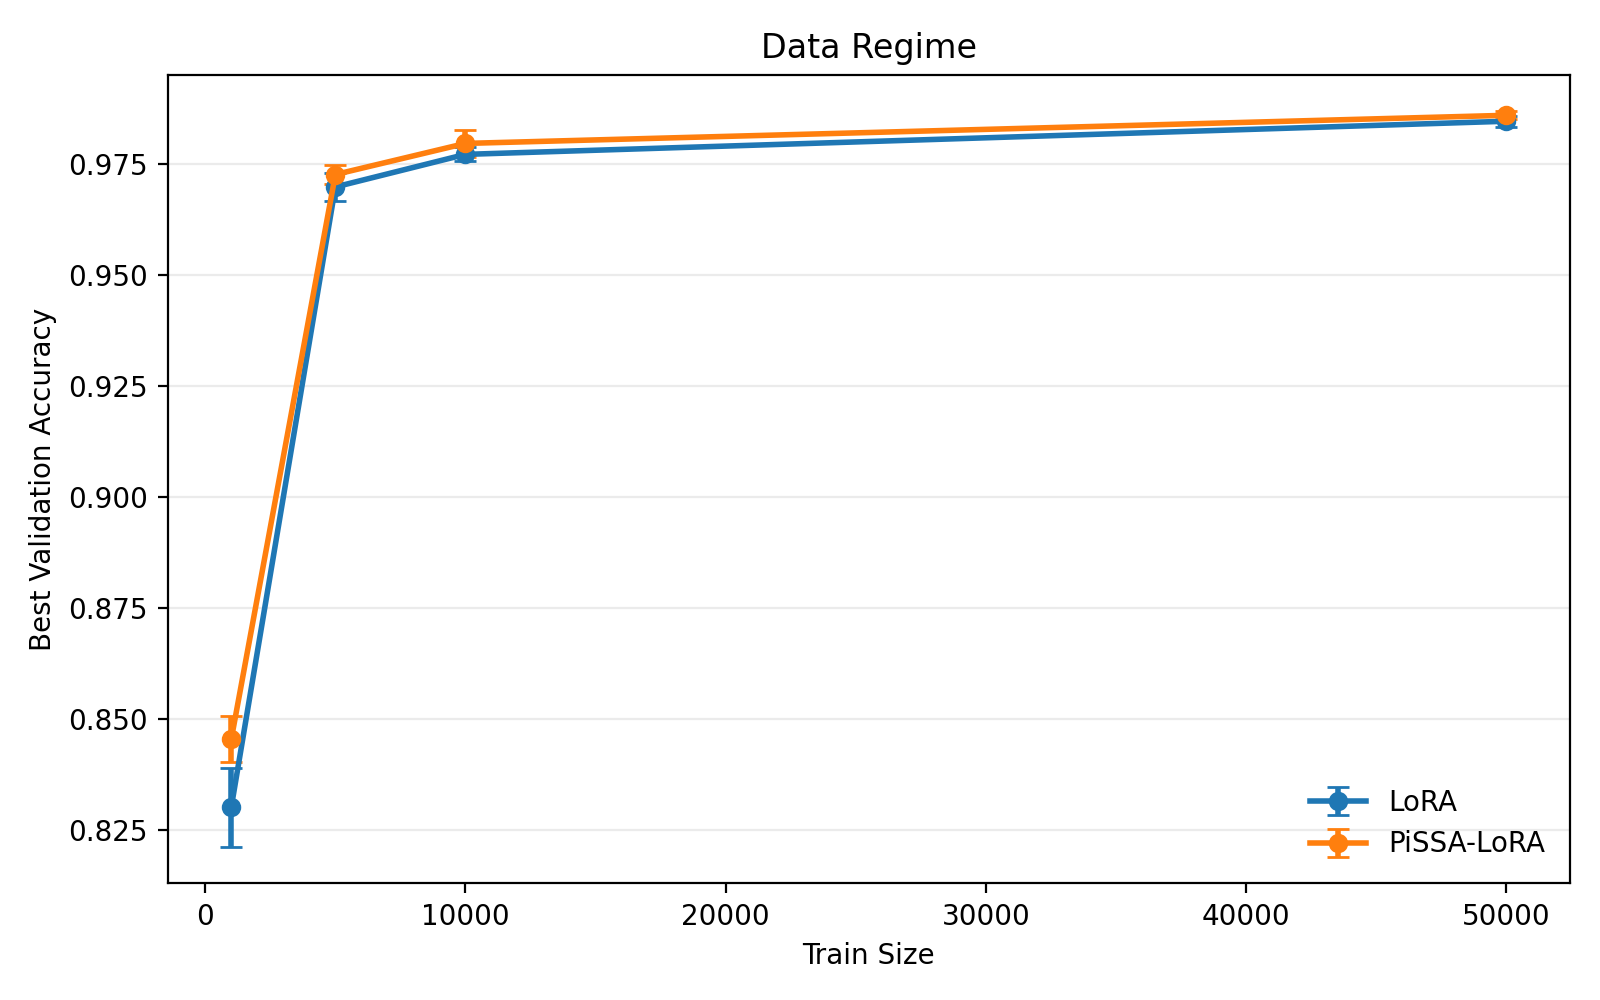
\includegraphics[width=0.95\linewidth]{figures/data_regime.png}
\end{center}
\caption{Mean best validation accuracy across data regimes. PiSSA-LoRA consistently beats standard LoRA, with the largest gain in the low-data regime.}
\label{fig:data-regime}
\end{figure}

This trend is important because it suggests \emph{when} PiSSA helps most. If the adapter initialization is more informative, the advantage should matter more when supervision is scarce and optimization is harder. That is exactly what we observe. At 50k examples, PiSSA-LoRA still improves over LoRA, but only by 0.13 points because the larger data budget reduces optimization sensitivity.

The strongest mean result in the entire study is obtained here: PiSSA-LoRA with 50k training images reaches 98.60\% $\pm$ 0.09, while standard LoRA reaches 98.47\% $\pm$ 0.13. The best single run is PiSSA-LoRA at 98.66\%.

\subsection{Rank Ablation}

Figure~\ref{fig:rank-ablation} studies whether the PiSSA advantage depends on LoRA rank. PiSSA-LoRA beats LoRA at all tested ranks. The largest gap appears at rank 16, where PiSSA-LoRA reaches 98.15\% $\pm$ 0.25 while LoRA reaches 97.67\% $\pm$ 0.11, a gain of 0.49 percentage points.

\begin{figure}[t]
\begin{center}
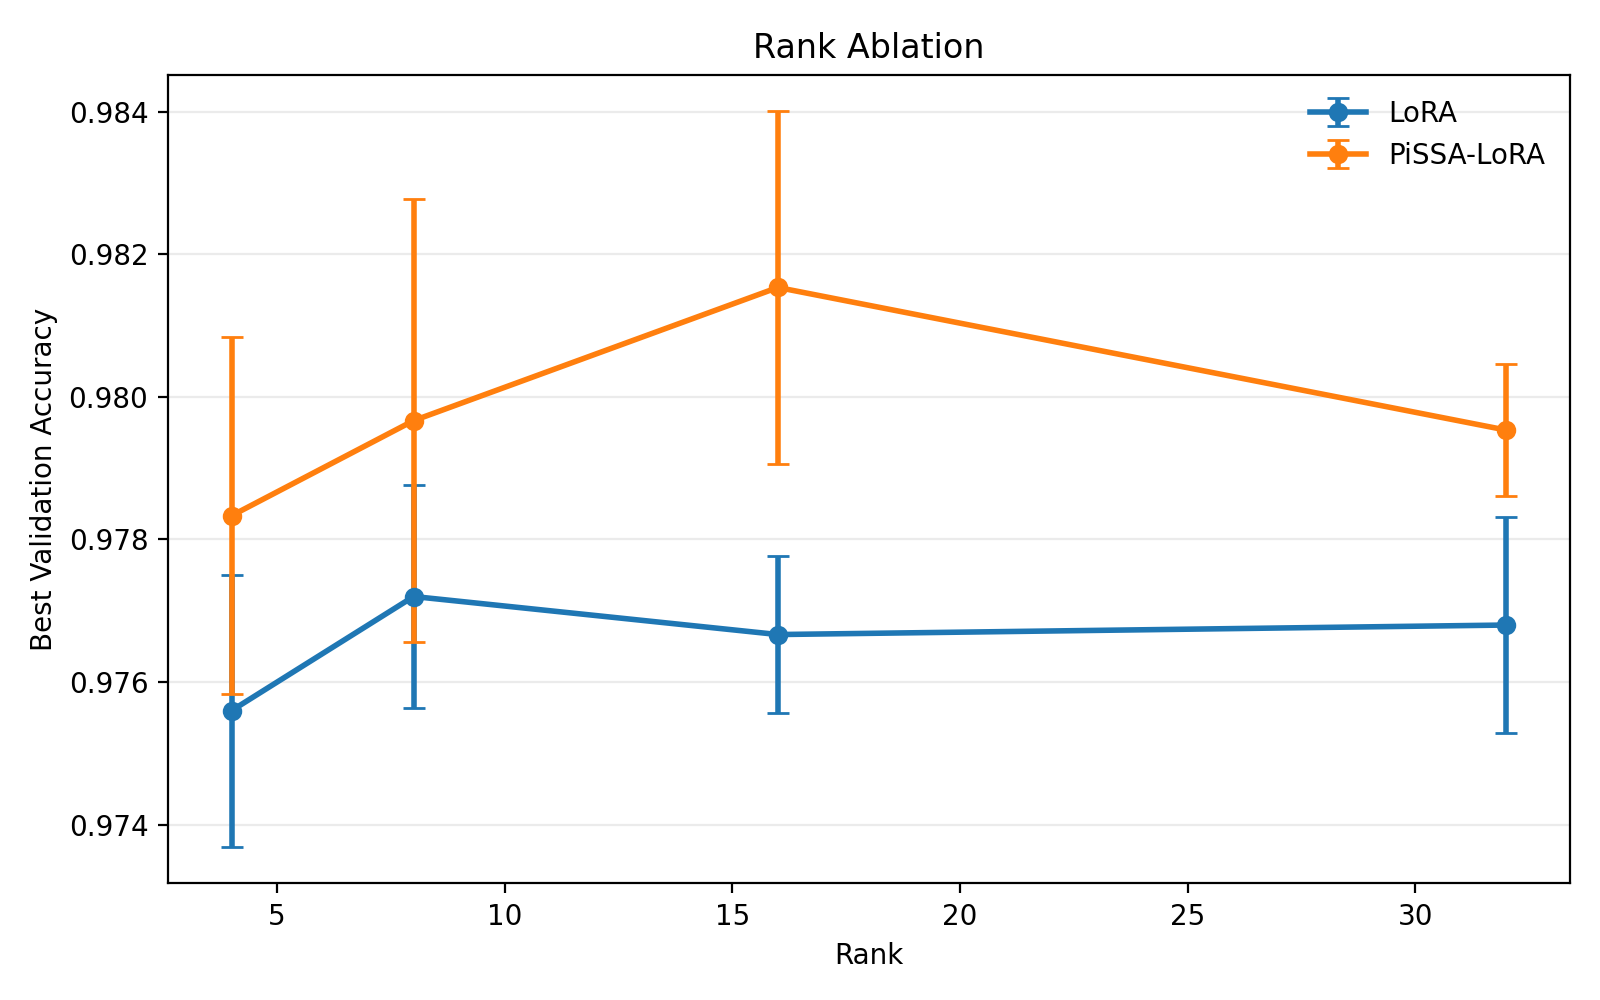
\includegraphics[width=0.95\linewidth]{figures/rank_ablation.png}
\end{center}
\caption{Mean best validation accuracy across adapter ranks. PiSSA-LoRA outperforms LoRA at every tested rank, with the best mean result at rank 16.}
\label{fig:rank-ablation}
\end{figure}

The rank sweep suggests that increasing rank from 4 to 8 helps both methods, but the best overall tradeoff appears at rank 16. Moving from rank 16 to 32 does not improve mean accuracy, even though the trainable parameter budget grows from 0.692\% to 1.365\% of the full model. This indicates diminishing returns at higher rank in this task.

\subsection{Discussion}

Taken together, the three suites tell a consistent story.

First, PiSSA-LoRA is the strongest method among the parameter-efficient alternatives, and it is even slightly better than full fine-tuning in the 5k quick ablation. Second, PiSSA's improvement is most meaningful in the low-data regime, which matches the intuition that better initialization matters most when data is limited. Third, a moderate adapter rank is enough: the best mean rank-ablation result comes from rank 16, not rank 32.

One nuance is that LoRA and PiSSA-LoRA do not always beat full fine-tuning in raw wall-clock time. On the H100 runs used here, full fine-tuning is slightly faster than the adapter methods in the small 5k experiment. The more compelling advantage of PiSSA-LoRA is therefore parameter efficiency and accuracy, not pure runtime reduction. For a course project, that is still a strong result because the rubric emphasizes functionality, relevance, and substantive evaluation rather than only the shortest training time.

\section{Conclusion}

This project reproduced and extended a PiSSA-style parameter-efficient fine-tuning study in a vision setting. The main contribution is a systematic empirical evaluation of PiSSA-LoRA for ViT fine-tuning on CIFAR-10, including multi-seed quick ablations, data-regime sweeps, and rank ablations. Across all three suites, PiSSA-LoRA consistently outperformed standard LoRA. In the 5k quick ablation it also slightly surpassed full fine-tuning while using roughly 284x fewer trainable parameters.

From a reproduction-track perspective, the project contributes two things. First, it verifies that PiSSA's main empirical advantage is not limited to the language-model domain in which it was introduced. Second, it provides a reproducible experiment pipeline, cluster-ready scripts, and a structured evaluation framework that goes beyond a minimal reimplementation. The results suggest that PiSSA-style initialization is a practical way to improve adapter tuning for vision transfer, especially when training data is limited.

\bibliographystyle{iclr2026_conference}
\bibliography{project_report}

\appendix
\section*{LLM Acknowledgement}

OpenAI Codex was used as a programming and writing assistant during this project. It helped restructure the experiment codebase, automate cluster runs, download and summarize result artifacts, and draft sections of the report. All experiment design choices, result selection, interpretation, and final submission decisions were reviewed and finalized by the author.

\end{document}
